\chapter{脉搏波的预处理及参数描述}
\section{引言}
前文已经阐述过,光电容积脉搏波(PPG)本身蕴含着丰富的血液动力学信息,其形态、强度、速率、节律等特征反映心脏的功能与状态,也可以反映出各级动脉及分支中血管壁弹性、血管阻力、血液黏度等信息。但同时,PPG信号也与其他医学电生理信号类似,
易收到多种噪声干扰。本章着重解决脉搏波信号的预处理问题与脉搏波描述等两个问题。针对前者,本章节阐述了信号处理一般过程,特别地,对如何提高脉搏波检测算法的精确性进行了多种创新机制的设计。针对后者,在介绍了脉搏波已有特征后,原创性地提出了多种
新型形态学时域特征,并在此基础上构建了脉搏波时域特征描述集合,为后续的分析打下坚实的基础。本章仅对以上内容进行原理及设计思路说明,相关的软件功能性设计可参阅本论文第六章节。
\section{信号预处理}
本小节着重解决如何提高原始信号质量并正确定位PPG相关特征点、检测完整脉搏波波形等内容。\autoref{fig:samplesignal}展示了一段有代表性的经由GE B650监护仪实际采集的PPG信号,从中可以看到所得信号整体信号质量较高,但仍然有基线偏移、
PPG信号重博波特征不明显等问题。这些问题可能与具体硬件检测电路、使用传感器种类及监护仪处理算法有关。此外,可以看到\autoref{fig:samplesignal}仍然有一段明显的无效数据段(约40s-55s期间内),在实际处理时需要对其进行剔除。
由于重博波特征不明显无法经由软件算法人工恢复,故本章节暂不对任何重博、切迹进行计算处理,后续也无任何与之相关的PPG信号特征参数。本章涉及的信号分析流程如\autoref{fig:process}所示。
\begin{figure}[htbp]
    \centering
    \includegraphics[width=\linewidth]{ch4/samplesignal}
    \caption{\label{fig:samplesignal}一名被试实采PPG信号(片段)}
\end{figure}
\begin{figure}[htbp]
    \centering
    
\includegraphics[width=\linewidth]{ch4/process.pdf}
    \caption{\label{fig:process}信号预处理流程示意}
\end{figure}

\subsection{信号滤波}
通常而言,数字滤波是生理信号处理的必不可少的过程,此前的诸多学者也在滤波处理领域提出了多种不同的滤波算法。但对本研究而言,由于临床标准监护仪导出所得的PPG信号质量高、干扰噪声较少,因此,本小节中仅使用了较为简单的5点滑动平均滤波器对其进行了处理。
若以$X$表示原始信号,$Y$表示滤波后信号,则有
\begin{equation}
    \label{equ:filter}
    Y(n)=\frac{X(n-2)+X(n-1)+X(n)+X(n+1)+X(n+2)}{5}
\end{equation}
经滑动滤波前后的PPG信号对比图如\autoref{fig:filter}所示。信噪比(signal-noise rate,SNR)与均方误差(root mean square error,RMSE)是最常用的评估滤波效果的两个指标,
\begin{equation}
    \label{equ:snr}
    SNR=10\log_{10}\frac{\sum_{i=1}^{n}{(X_i-\mathop{X} \limits^-})^2}{\sum_{i=1}^{n}{(X_i-Y_i})^2}
\end{equation}
\begin{equation}
    \label{equ:rmse}
    RMSE=\sqrt{\frac{\sum_{i=1}^{n}{(X_i-Y_i})^2}{n}}
\end{equation}
对\autoref{fig:filter}信号段进行检测,可得$SNR=33.19$,$RMSE=6.27$。此时,PPG信号波形特征已比较清晰,可以满足后续分析需求。
\begin{figure}[htbp]
    \centering
    \subfigure[原始PPG信号]{
    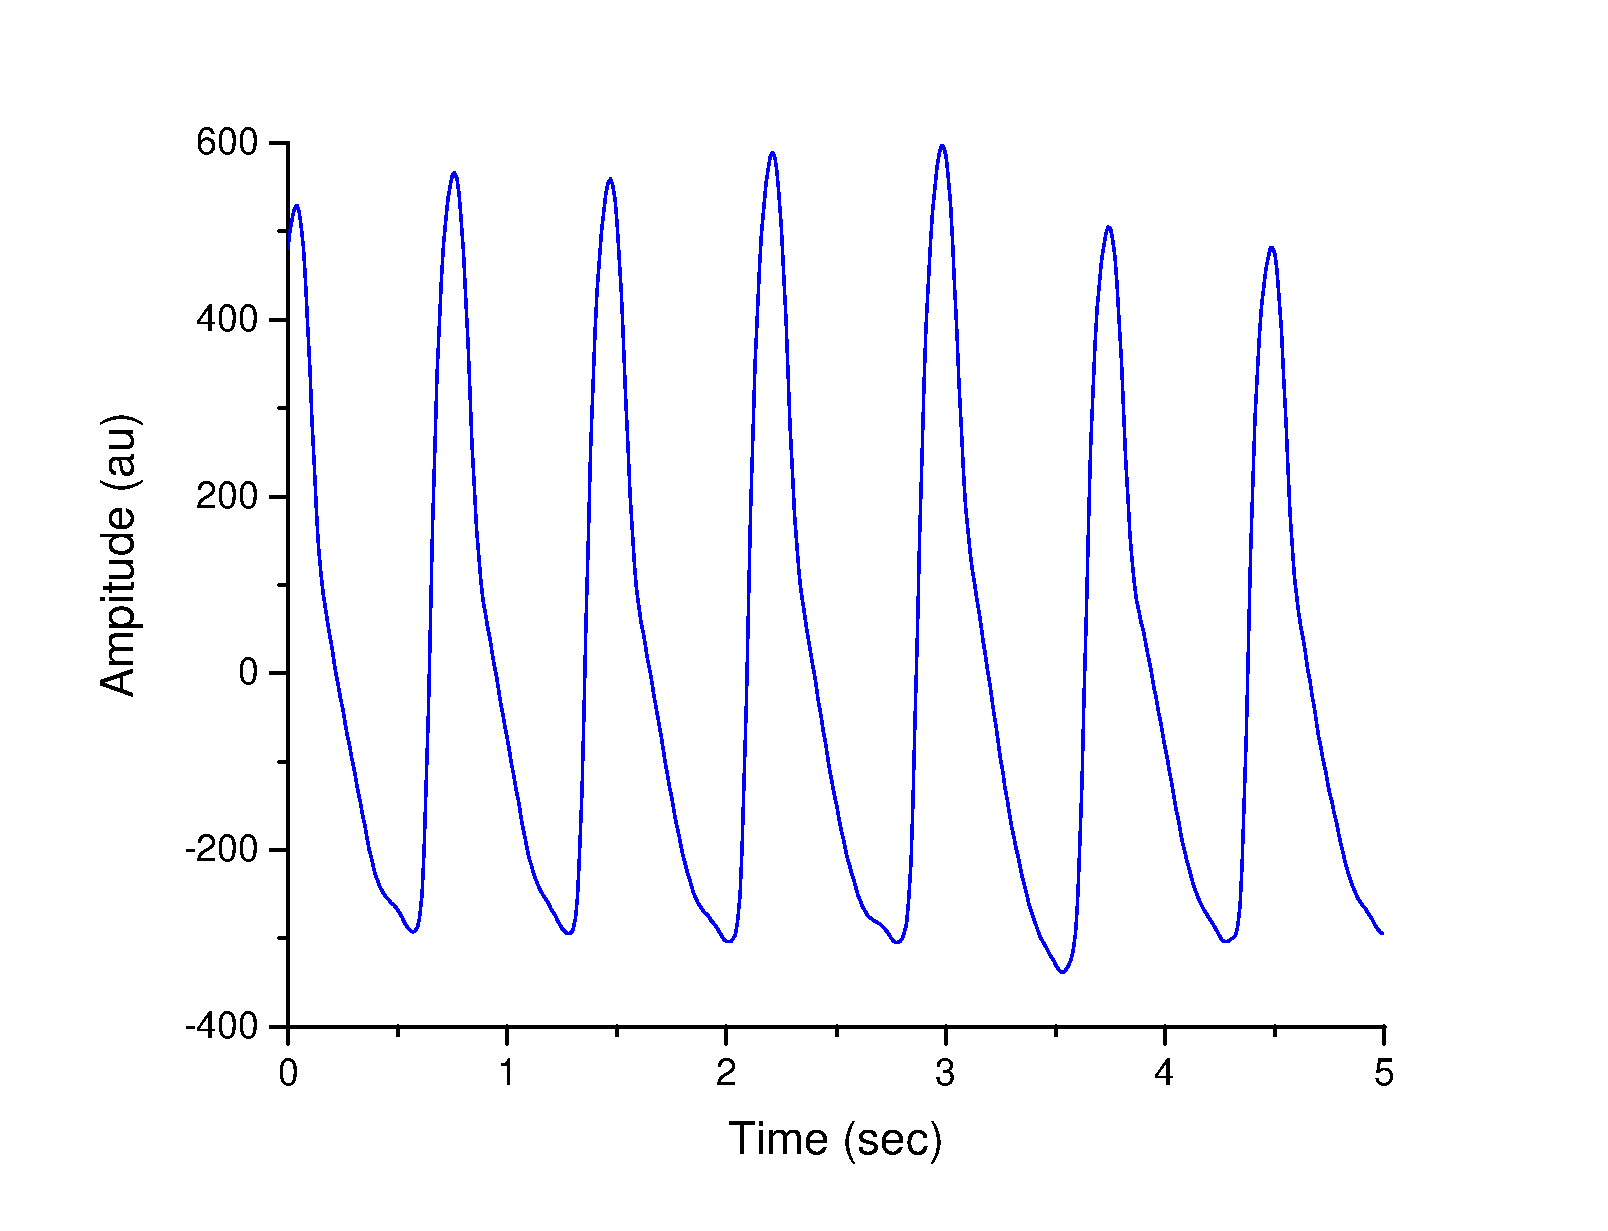
\includegraphics[width=6cm]{ch4/before}
    }
    \quad
    \subfigure[平滑滤波后PPG信号]{
    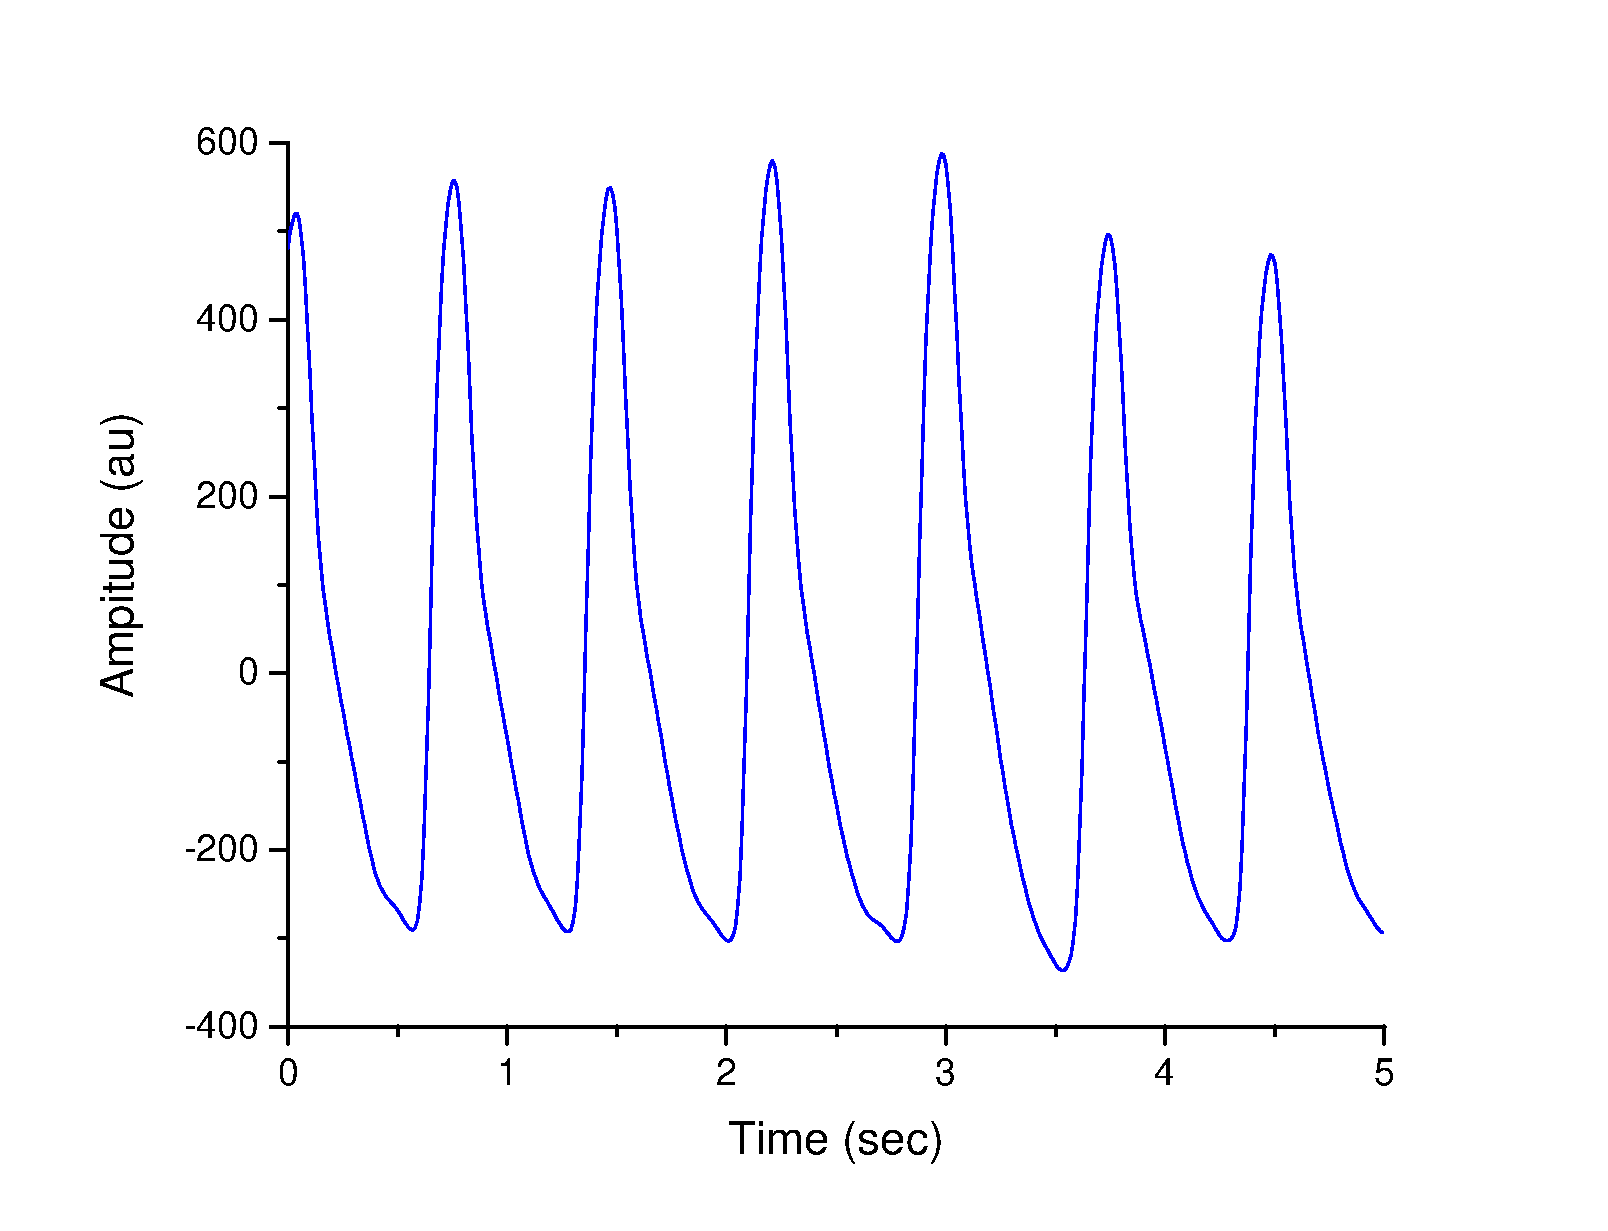
\includegraphics[width=6cm]{ch4/after}
    }
    \caption{\label{fig:filter}平滑滤波前后PPG信号对比}
\end{figure}

\subsection{波形检测}
脉搏波波形的正确检测是后续所有特征计算的基础,波形检测的准确性及抗干扰能力显得尤为重要。传统的波形检测一般都是对波形进行一次性检测,然后再人工判别检测的准确性。本小节则改进了这一流程,提出了PPG波形的初筛-复核-
投票(Screen-Check-Vote,SCV)算法。具体而言,SCV算法充分利用“宽进严出”的筛选原则,依据PPG波峰的局部最大值原理进行波形初筛,随后特创新性地引入了针对PPG波形的多标准二次复核与最终决策确认机制以减少错检发生的概率。
所有初筛得到的“可疑波形”经特定标准复核后均会得到基于该标准的一个输出判定结果。最后,由检测算法的决策模块负责对多个标准的复核结果进行裁决判定,将“可疑波形”判断识别为正确波形或错检干扰段。上述复合检测过程如\autoref{fig:detect}所示。
\begin{figure}[htbp]
    \centering
    
\includegraphics[width=\linewidth]{ch4/detect}
    \caption{\label{fig:detect}波形检测流程示意}
\end{figure}

一、波形检测

波峰与波谷是脉搏波的最基本特征点,也是检测波形其他特征点的基础。顾名思义,波峰是特定PPG波形内的最大值,在其左邻域内PPG幅值单调递增,右邻域内PPG幅值单调递减,则显然波峰与波谷必然是原始数据中的局部极大值与局部极小值点。
故对PPG波形特征点定位可按以下步骤进行。

1. 波峰波谷定位

计算并遍历原始信号的一阶导数$X^{'}$,若出现$X_i^{'}\ge 0$且$X_{i+1}^{'}\le 0$,则说明出现了极大值。此时,定义时长一长一短的两个搜索窗,分别以当前数据点为窗中心,向前后双向检测并返回窗内最大值的位置。
若两个搜索窗的返回结果一致,则说明返回值就是一个波峰点。为防止同一波峰被多次检测,只有与上一成功检测的波峰位置点不同返回值才会被加入波峰缓存数组$Peaks$中。

在实际检测时,常会出现一阶导数在某邻域内多次出现过零点,导致多个极大极小值连续出现。为避免连续调用搜索窗、提高算法效率,本研究针对性进行了如下剪枝设计:

\Rnum{1}.采用中心对称搜索窗

窗口进行最大值搜索时是以当前搜索位置中心对称前后双向搜索,实际当第一个过零点出现时,这一邻域内的所有极值点均已被检索过,得到的局部最值已经是该邻域内最值。

\Rnum{2}.合理设置搜索窗时长

结合正常波形的形态特点,本研究将搜索窗时长分别设置为0.1s与0.3s。前者可以直接剔除掉时间跨度过小的局部极值,后者是基于此前PPG波峰与其重博峰时间间隔的经验值,可以保证重博峰点不会被误检为整个波形的波峰。

\Rnum{3}.搜索窗步进值策略调整

若长窗在当前位置$C$以中心沿时间轴延伸方向找到了局部极大值的坐标$L$后,下一次的搜索窗位置可直接从该$L$处开始。具体而言,若此时短窗返回结果$S=L$,则返回值必然是检测得到的波峰位置$P$,下次搜索可直接从波峰后开始;若$S\ne L$,
此时从$C$至$L$再进行搜索已经不可能再更新$L$坐标。而由于长窗搜索必然包含短窗,故下次搜索也可以同样调整检索位置从$L$处开始。

对波谷的定位可参考上述波峰定位过程稍加修改后在一遍遍历中一同完成。类似地,波谷位置也被保存至缓存数组$Troughs$中。

2. 完整波形确认

由于上一步已经分别得到了原始信号中所有波峰与波谷点,为方便后续研究,此时仅需按照波谷(start)——波峰(peak)——下一波谷(end)组合成完整波形即可。参考以往研究对PPG波形对经验统计,本研究规定,波形起点与波形终点间期$P_{S2E}\ge 0.4s$,
波形峰值点与波形终点间期$P_{P2E}\ge 0.3s$。只有满足了该PPG间期的波形才是检波算法初检合格的输出。

% 这一过程如\autoref{alg:detect}所示。
% \begin{breakablealgorithm}
%     \caption{PPG信号检测特征点检测}
%     \label{alg:detect}
%     \begin{algorithmic}[1] %每行显示行号
%         \Require 待检原始数据数组$Points$,数组大小$n$,原始采样率$samplerate$
%         \Ensure 包含起始点及峰值点坐标的所有初筛合格的波形
%         \Function {Detect}{$Points, samplerate$}
%             \State 初始化$pulse$
%             \If {$left < right$}
%                 \State $middle \gets (left + right) / 2$
%                 \State $result \gets result +$ \Call{MergerSort}{$Array, left, middle$}
%                 \State $result \gets result +$ \Call{MergerSort}{$Array, middle, right$}
%                 \State $result \gets result +$ \Call{Merger}{$Array,left,middle,right$}
%             \EndIf
%             \State \Return{$pulse$}
%         \EndFunction
%     \end{algorithmic}
% \end{breakablealgorithm}

二、多标准评估

对正常PPG波形,上述检测算法可以实现较好的检测效果,但对类似\autoref{fig:samplesignal}中的无效数据段信号极易产生错误识别与检测。为增强算法对干扰信号的检测能力、对畸变信号的识别判断能力,本研究引入了对PPG波形对二次审核评估机制。
由于本研究中采集得到的PPG信号不存在运动伪差干扰,所有有效PPG波形信号在理论上应具有较高的相似性。此外,有效PPG信号与干扰信号、畸变信号在形态特征、统计特征方面均存在较大差异,存在设计算法实现自动区分的理论可行性。基于以上前提,
为使具有且仅具有PPG波形一般特征的初筛“可疑波形”可以通过复核评估,本研究特设计并提出了以下复核标准。

1.能量与功率标准

易知脉搏波的相对幅值$A$是采样时间$t$的函数,将其表示为$A(t)$。参考信号与系统中对时间信号能量的定义\cite{Alan2019},则单个PPG信号的能量可表示为
\begin{equation}
    \label{equ:ppge}
    E=\sum_{t=t_{start}}^{t_{end}}|A(t)|^2
\end{equation}
同理可得该PPG波形在其持续时间内的平均功率为
\begin{equation}
    \label{equ:ppgp}
    P=\frac{E}{t_{end}-t_{start}}=\frac{\sum_{t=t_{start}}^{t_{end}}|A(t)|^2}{t_{end}-t_{start}}
\end{equation}
能量标准基于PPG波形在原始采集数值上(包含PPG信号中AD成份)的相似性。所有初筛波形功率求其均值,可得筛选波形的平均功率$P_{mean}$。本研究规定通过能量标准复核的波形其功率必须在$P_{mean}$的一定倍数区间内$[0.5P_{mean},1.5P_{mean}]$。

2.方差与标准差标准

若原始PPG信号中AD成份波动较大(如基线严重漂移),会使部分波形功率数值偏离上述正常$P_{mean}$合理倍数区间,导致这部分波形被能量与功率标准错误识别为干扰。因此,本研究引入了方差与标准差标准以重点关注PPG波形AC成份的相似性。
若将特定PPG波形持续时间内所有采样点均值定义为$\mathop{A} \limits^-$,则该波形的标准差可表示为
\begin{equation}
    \label{equ:ppgstd}
    S=\sqrt{\frac{\sum_{i=1}^{n}{(A_i-\mathop{A} \limits^-})^2}{n}}=\sqrt{\frac{\sum_{i=1}^n{A_i}^2}{n}-{\mathop{A} \limits^-}^2}
\end{equation}
类似地,可以计算所有初筛波形的标准差均值为$S_{mean}$。本研究规定通过标准差复核的波形其标准差必须在$S_{mean}$的一定倍数区间内$[0.5S_{mean},1.5S_{mean}]$。

3.时间关系标准

时间关系标准是对PPG波形间期、波形上升支与下降支及重博波峰相关特征时长间期做出对限定。由于时间标准可在波形特征点定位后直接计算,且是合格波形筛查所共有的范式。因此,本研究直接将时间标准应用于波形检测初筛阶段,
如搜索窗对时间设置已经限定了重博波峰与主波峰间期为$T_{P2R}\ge0.3s$、
波形在进行确认时也限定了波形周期$T_{S2E}\ge 0.4s$、下降支时长$T_{P2E}\ge 0.3s$。若参照心率定义,将一分钟中内有效脉搏波的数量规定为脉率(Pulse Rate,PR)。那么,原则上该算法可对$PR \le 150$的原始脉搏波数据进行波形检测。
而在实际检测过程中,可视具体信号质量对上述时间标准中的参数进行调整以完成算法的适配。

4.基线偏移标准

基线偏移最值标准是对PPG波形的起点与终点幅值差异程度的衡量,若两者的差值过大基线漂移严重,则说明该波形很可能处于一段干扰中,如\autoref{fig:samplesignal}中约37s-45s期间的信号。
若规定PPG波形起点与终点中幅值的较大的为$A_G$,较小值为$A_L$,同时规定波峰幅值为$A_P$,则基线偏移程度可用以下公式衡量
\begin{equation}
    \label{equ:baselinestd}
    \left \{
    \begin{aligned}
        \delta B &=A_G-A_L \\
        \Delta B &=\frac{A_G-A_L}{A_P-A_L}=\frac{\delta B}{A_P-A_L}
    \end{aligned}
    \right.
\end{equation}
其中,$\delta B$是对偏移的绝对值的衡量,$\Delta B$则是对偏移程度归一化的衡量。本研究采用$\Delta B$对PPG波形进行筛选。由于正常PPG波形$\Delta B$数值较小,而基线严重漂移时$\Delta B$数值显著增大,甚至达到正常波形的数十倍以上。
为消除漂移波形对最终均值的影响,本研究在计算出所有波形的$\Delta B$数值并按升序排列后,取前$80\%$的波形计算其均值${\Delta B}_{mean}$。
本研究规定通过基线偏移复核的波形其$\Delta B$数值必须在${\Delta B}_{mean}$的一定倍数区间内$[0,10{\Delta B}_{mean}]$。

5.其他标准

目前为空,待补充。由于不同人群、不同采集设备、不同采集环境下采集得到的PPG信号可能形态上千差万别,同时干扰信号也往往不尽相同。上述标准仍有不足以甄别区分有效信号与无效干扰的可能。
故在此特保留其他标准占位,供后续研究视情况开发设计新标准从而进行功能性拓展。

三、投票决策

当上述多个PPG波形评估器构建完成后,对PPG初筛待检波形均会生成一定的输出——正确检测波形或错检干扰。该过程可抽象成使用多个学习器$h_i$从类别标记集合$\{c_0,c_1,\cdots,c_N\}$中产生最终输出。则此时可借鉴集成学习中的投票策略(voting)完成对初筛波形的最终判别
决策\cite{Zhou2016}。若将$h_i$在样本$x$上的预测输出表示为$N$维向量$(h_i^1(x);h_i^2(x);\cdots;h_i^N(x))$,则常见可用的投票策略包含以下三种\cite{Kittler1998,Zhou2016}:

1.绝对多数投票法

若某标记得票数超过半数,则预测为该标记,否则拒绝该预测。
\begin{equation}
    \label{equ:mvoting}
    H(x)=
    \left \{
    \begin{aligned}
        c_j,&\quad if \sum_{i=1}^T{h_i^j(x)}>0.5\sum_{k=1}^N{\sum_{i=1}^T}{h_i^k(x)}\\
        reject,&\quad otherwise.
    \end{aligned}
    \right.
\end{equation}

2.相对多数投票法

应用绝对多数投票法时,若对所有标记类别,其得票数均不超过半数,则此时无法得出投票结果。为避免此情况发生,相对多数投票法直接将预测为得票最多的标记。若同时有多个标记获得最高票,则从中随机选取一个作为最终结果。
\begin{equation}
    \label{equ:pvoting}
    H(x)=c_{\arg \max\limits_{j} \sum_{i=1}^T{h_i^j(x)}}
\end{equation}

3.加权投票法

与前面两种投票法不同,加权投票法给所有的学习器$h_i$以特定的权重$w_i$,将所有可能汇总后得到最后的标记类别,
\begin{equation}
    \label{equ:wvoting}
    H(x)=c_{\arg \max\limits_{j} \sum_{i=1}^T{w_ih_i^j(x)}}
\end{equation}
其中,$w_i\ge0$,$\sum_{i=1}^T{w_i=1}$。
\begin{table}[htbp]
    \centering
    \caption{\label{tab:vote}类标记与类概率特点对比}
    \begin{tabularx}{\linewidth}{c|X<{\centering}X<{\centering}}
        \Xhline{1pt} 
            &\textbf{类标记}&\textbf{类概率}\\
        \hline
        \textbf{$h_i^j(x)$值域}  &$\{0,1\}$    &$[0,1]$     \\
        \textbf{$h_i^j(x)$输出说明}&\tabincell{c}{若$h_i$将样本$x$预测为$c_j$\\则取值为1,否则为0}&\tabincell{c}{$h_i^j(x)$相当于对后验概率\\$P(c_j|x)$的一个估计}\\
        \textbf{投票策略}&\tabincell{c}{绝对多数投票法、\\相对多数投票法}&加权投票法\\
        \textbf{别称}    &硬投票 &软投票 \\
        \Xhline{1pt}
    \end{tabularx}
\end{table}

\autoref{equ:mvoting}至\autoref{equ:wvoting}并没有限制单个学习器输出值类型,而常见的学习器输出值$h_i^j(x)$有类标记与类概率两大类。而基于这两类输出值进行的投票也相应被称为硬投票与软投票,类标记与类概率的特点可总结概括为\autoref{tab:vote}所示。
需要注意的是,硬投票可能会导致最终的分类结果由多数概率值较低的学习器决定,而非少数概率更高、更有分类把握的学习器。因此,在条件允许的情况下,应尽可能使用软投票机制进行决策。

由于本研究尚未对上述PPG波形评估器的类概率进行相关研究,因而选择将各评估器的输出暂时直接限定为类别标记输出为0或1,最终基于硬投票策略进行初筛波形的类型判别。

四、检测算法性能评估

PPG波形特征点按上述SCV算法定位完成后,需要对算法的性能进行分析评估。仍以\autoref{fig:samplesignal}中实采信号为例,利用SCV算法对其进行检测,初筛结果如\autoref{fig:detectcheck}所示,图中波峰处数字为该波形的初筛编号。
可以看到SCV算法并不保证检测波形在时间上的连续性,在初筛阶段就会忽略明显不符合时间标准的PPG数据段,如\autoref{fig:detectcheck}中44s-60s间的多段数据。而在初筛结果中,肉眼可辨别的明显异常的波形也在复核阶段被检测并经投票
最终判定,如\autoref{tab:detect}所示。其中,输出值为0代表该初筛波形被判定为正常波形,否则为干扰段;加权投票输出是将功率标准、标准差标准及基线标准按0.4、0.4与0.2的权重计算,并将计算结果超过0.5的判定为干扰段得到的;
人工裁定一栏是由临床医生与科研人员集体讨论后对待审核PPG波形做出的判定,是本研究用以评估算法性能的“金标准”。
\begin{figure}[htbp]
    \centering
    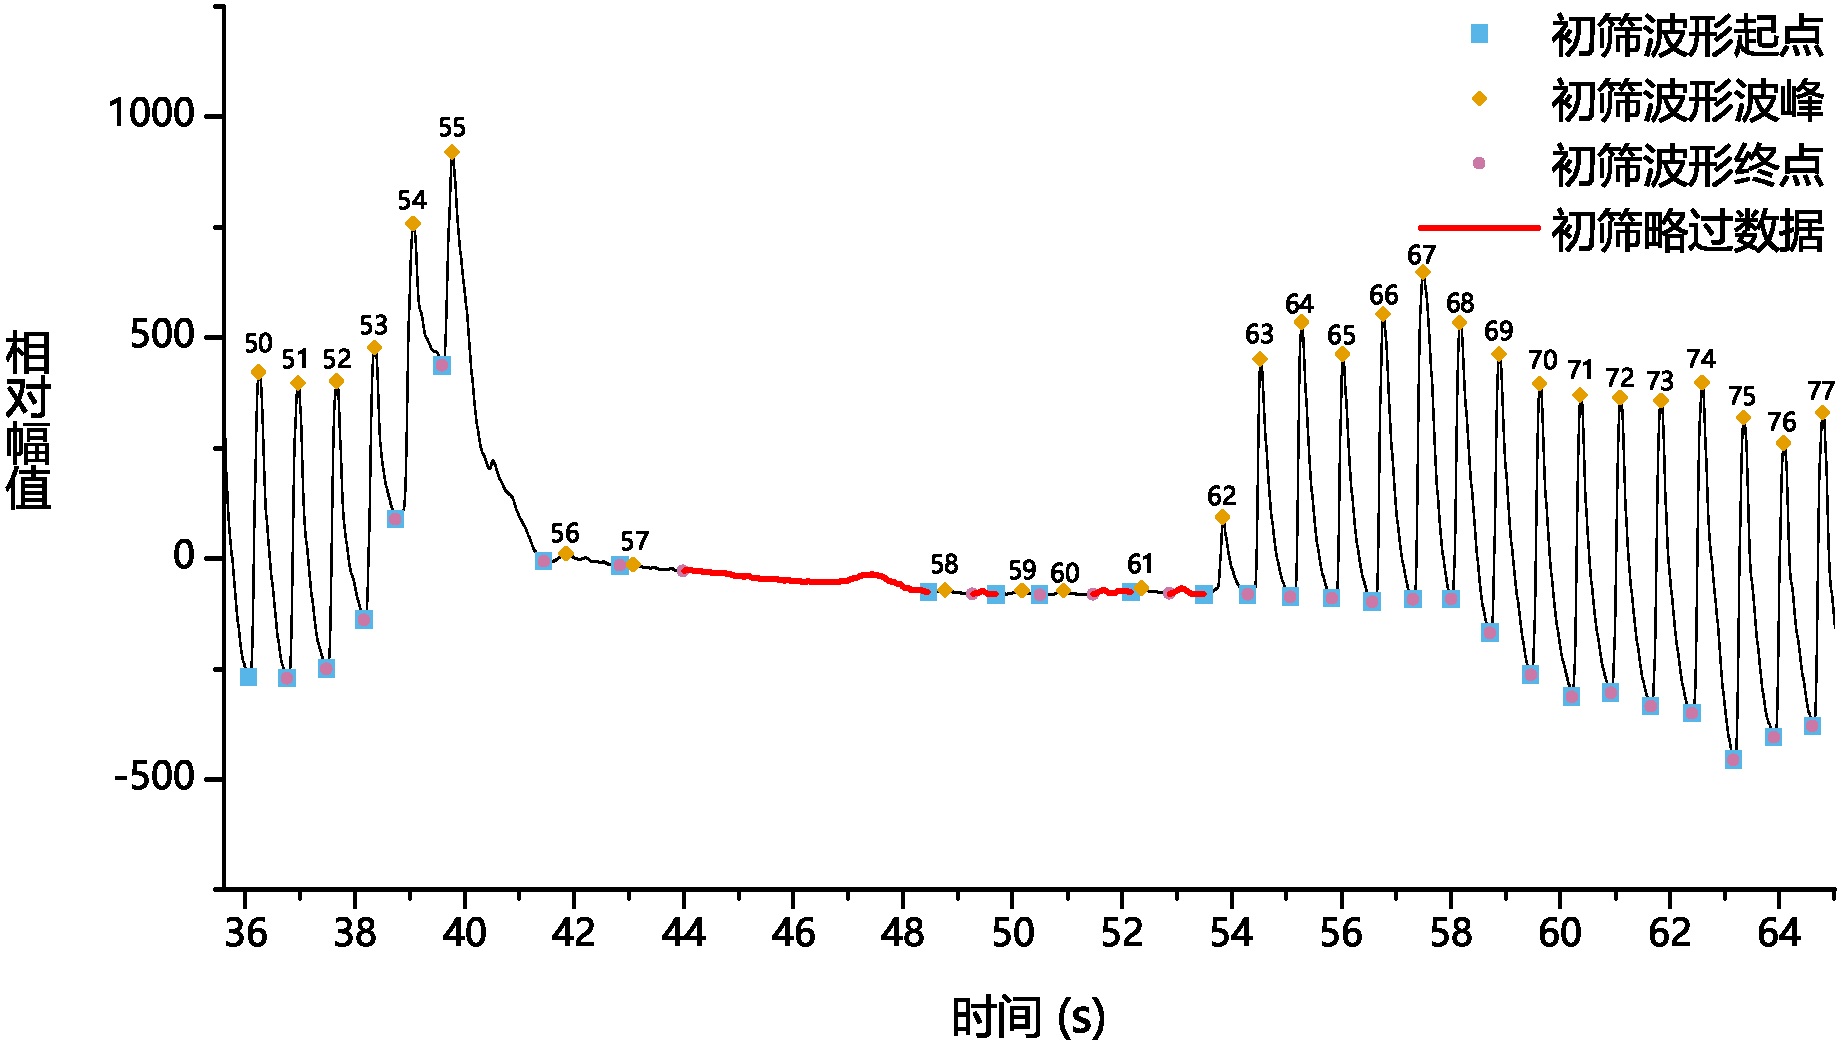
\includegraphics[width=0.9\linewidth]{ch4/detectcheck}
    \caption{\label{fig:detectcheck}PPG波形检测算法初筛结果}
\end{figure}

\autoref{fig:samplesignal}中初筛波形共有114个,对\autoref{tab:detect}中涉及的三种复核标准与两种投票结果使用混淆矩阵分析可得到各标准、投票的性能表现如\autoref{tab:checkevaluation}所示。
可以看到复核模块的各审核单项标准均有着较好的识别纠错能力,单项准确性均在95\%以上,特异性更是均在99\%以上。值得一提的是,复核标准功率与标准差在定义上就有着极高的相似性,检测结果也十分相近。
对本测试数据而言,功率标准有着更高的灵敏度(100\%),能够把所有干扰段全部有效识别(挑得全但有挑错);而标准差则有着更高的精准率(100\%),能够保证识别出的全部都是干扰段(挑得少但挑得准)。
\begin{table}[htbp]
    \centering
    \caption{\label{tab:detect}SCV算法对初筛波形的复核及决策输出(局部)}
    \begin{tabularx}{\linewidth}{X<{\centering}ccccX<{\centering}cX<{\centering}X<{\centering}}
    \toprule
    \multirow{2}[4]{*}{\textbf{波形编号}} & \multicolumn{3}{c}{\textbf{单项复核评估标准输出}} & \multicolumn{2}{c}{\textbf{绝对多数投票}} & \multicolumn{2}{c}{\textbf{加权投票}} & \multirow{2}[2]{*}{\textbf{人工裁定}}\\
    \cmidrule{2-8} & \textbf{功率} & \textbf{标准差} & \textbf{基线} & \textbf{输出} & \textbf{判定} & \textbf{输出} & \textbf{判定} \\
    \midrule
    ……    & ……    & ……    & ……    & ……    & ……    & ……    & …… & ……\\
    52    & 0     & 0     & 0     & 0     & 正常波形  & 0     & 正常波形 & 正常波形\\
    53    & 0     & 0     & 1     & 0     & 正常波形  & 0.2   & 正常波形 & 正常波形\\
    54    & 1     & 0     & 1     & 1     & 干扰段   & 0.6   & 干扰段 & 干扰段\\
    55    & 1     & 0     & 1     & 1     & 干扰段   & 0.6   & 干扰段 & 干扰段\\
    56    & 1     & 1     & 1     & 1     & 干扰段   & 1     & 干扰段 & 干扰段\\
    57    & 1     & 1     & 1     & 1     & 干扰段   & 1     & 干扰段 & 干扰段\\
    58    & 1     & 1     & 1     & 1     & 干扰段   & 1     & 干扰段 & 干扰段\\
    59    & 1     & 1     & 0     & 1     & 干扰段   & 0.8   & 干扰段 & 干扰段\\
    60    & 1     & 1     & 1     & 1     & 干扰段   & 1     & 干扰段 & 干扰段\\
    61    & 1     & 1     & 0     & 1     & 干扰段   & 0.8   & 干扰段 & 干扰段\\
    62    & 1     & 1     & 0     & 1     & 干扰段   & 0.8   & 干扰段 & 干扰段\\
    63    & 1     & 1     & 0     & 1     & 干扰段   & 0.8   & 干扰段 & 干扰段\\
    64    & 0     & 0     & 0     & 0     & 正常波形  & 0     & 正常波形 & 正常波形\\
    ……    & ……    & ……    & ……    & ……    & ……    & ……    & …… & ……\\
    80    & 1     & 0     & 0     & 0     & 正常波形  & 0.4   & 正常波形 & 正常波形\\
    ……    & ……    & ……    & ……    & ……    & ……    & ……    & …… & ……\\
    \bottomrule
    \end{tabularx}%
\end{table}%

此外,\autoref{tab:checkevaluation}中结果还表明,两种投票决策机制对本测试数据表现堪称完美,均能对PPG信号中干扰实现完美甄别。这也从侧面说明现阶段采用的功率、标准差、时间与基线等四个复核标准
设计合理,使用较少的决策变量即可满足本研究的处理任务,达到预期甄别目的。另一方面,上述结果也表明,与绝对多数投票机制对比,加权投票的性能优势尚充分发挥。
若待处理信号相对复杂、干扰严重,随着筛选标准的增多,各标准对最终判别的影响程度不同,此时对各指标的加权系数进行调整优化后,加权投票的性能优势就可以凸显。
\begin{table}[htbp]
    \centering
    \caption{\label{tab:checkevaluation}SCV算法的复核标准及决策机制性能评估}
    \begin{tabularx}{\linewidth}{cccccX<{\centering}X<{\centering}X<{\centering}X<{\centering}}
        \toprule
        \textbf{标准/机制}&\textbf{TP}&\textbf{FP}&\textbf{FN}&\textbf{TN}&\textbf{准确率}&\textbf{精准率}&\textbf{灵敏度}&\textbf{特异度}\\
        \midrule
            功率    & 10    & 1     & 0     & 103   & 99.1\% & 90.9\% & 100.0\% & 99.0\% \\
            标准差   & 8     & 0     & 2     & 104   & 98.2\% & 100.0\% & 80.0\% & 100.0\% \\
            基线    & 6     & 1     & 4     & 103   & 95.6\% & 87.5\% & 60.0\% & 99.0\% \\
            绝对多数投票 & 10    & 0     & 0     & 104   & 100.0\% & 100.0\% & 100.0\% & 100.0\% \\
            加权投票  & 10    & 0     & 0     & 104   & 100.0\% & 100.0\% & 100.0\% & 100.0\% \\
        \bottomrule
    \end{tabularx}
\end{table}

综上所述,SCV算法在PPG波形检测问题上的检测性能优异,抗干扰能力强。其中,SCV算法复核阶段各检测标准设计合理,均可按照设计初衷识别出特定的异常干扰段。同时,由于SCV算法整体采用模块化设计,各模块均具有良好的拓展性,
不论是对已获取的数据进一步提高检测性能,还是对新的存在特定干扰待检信号的准确检测,SCV算法都有着可进一步挖掘的潜力。

\subsection{重搏波与切迹检测}
重博波是脉搏波最具标志性的波形特征之一,重博波波峰与切迹的检测是一个完整的脉搏波检测算法必不可少的定位项之一\cite{Wang2012}。但在实际应用中,并不是每个人的PPG信号都有着明显的重搏波,特别是当被试出现外周阻力增加、血管壁弹性下降的情况后\cite{mmt}。
此时,随着PPG波形向外周传播,尖锐的重搏波切迹(incisura)常会变形甚至丢失,退变成一简单拐点,甚至重搏波波峰都会在下降支中不显著,导致最后无法从采集得到的信号中对两者直接进行精准定位,如\autoref{fig:samplesignal}所示。

针对重搏波与切迹不明显的PPG原始信号,本研究借鉴使用了王选等人于2012年提出的一种基于曲率的定位算法\cite{Wang2012},其核心思想是PPG信号在切迹退化成的变形点的邻域内具有最大的曲率值。在数学中,一般将曲线函数在点$(x,y)$处的曲率$K$定义为
\begin{equation}
    \label{equ:curvature}
    K=\frac{|y^{''}|}{{(1+{y^{'}}^2)}^{3/2}}
\end{equation}
其中,$y^{'}$与$y^{''}$分别是曲线函数在该点的一阶导数与二阶导数。如\autoref{fig:incisura}所示,该算法检测过程可概括如下:
\begin{figure}[htbp]
    \centering
    \includegraphics[width=.6\linewidth]{ch4/incisura}
    \caption{\label{fig:incisura}重搏波及切迹定位原理}
\end{figure}

首先,遍历切迹可能出现的所有位置,即PPG波形的下降支中后部分约$[\frac{3}{10}-\frac{9}{10}]$区间内。将该区间内一阶导数取值最大的点记为$M$,并对点M处的一阶导数$Y_M^{'}$的数值进行判断。

若$Y_M^{'}\ge 0$,说明在下降支中一定存在一段单调上升的波形,即存在明显的重搏波。此时,重搏波波峰即为点M至脉搏波终点之间的极大值点,切迹为脉搏波波峰至点M之间的最小值点。

若$Y_M^{'}<0$,说明脉搏波下降支一直单调下降,即不存在明显的重搏波。此时,可将重搏波波峰定义为点M至脉搏波终点之间的曲率最大处,切迹定义为脉搏波波峰至点M之间的曲率最小处。
\subsection{去除基线漂移}
在实际得到的PPG波形中,由于呼吸干扰等原因,一个完整PPG波形对应的两个波谷,即该波形的始末位置的幅值很难保持一致。这种差异最终会导致PPG信号的基线出现波动,也就是工程领域的基线漂移问题,如\autoref{fig:drift}所示。为满足后续特定PPG形态特征计算需求,
需要消除基线漂移的影响。此时一种基于线性变换的处理过程可以实现该目标。
\begin{figure}[htbp]
    \centering
    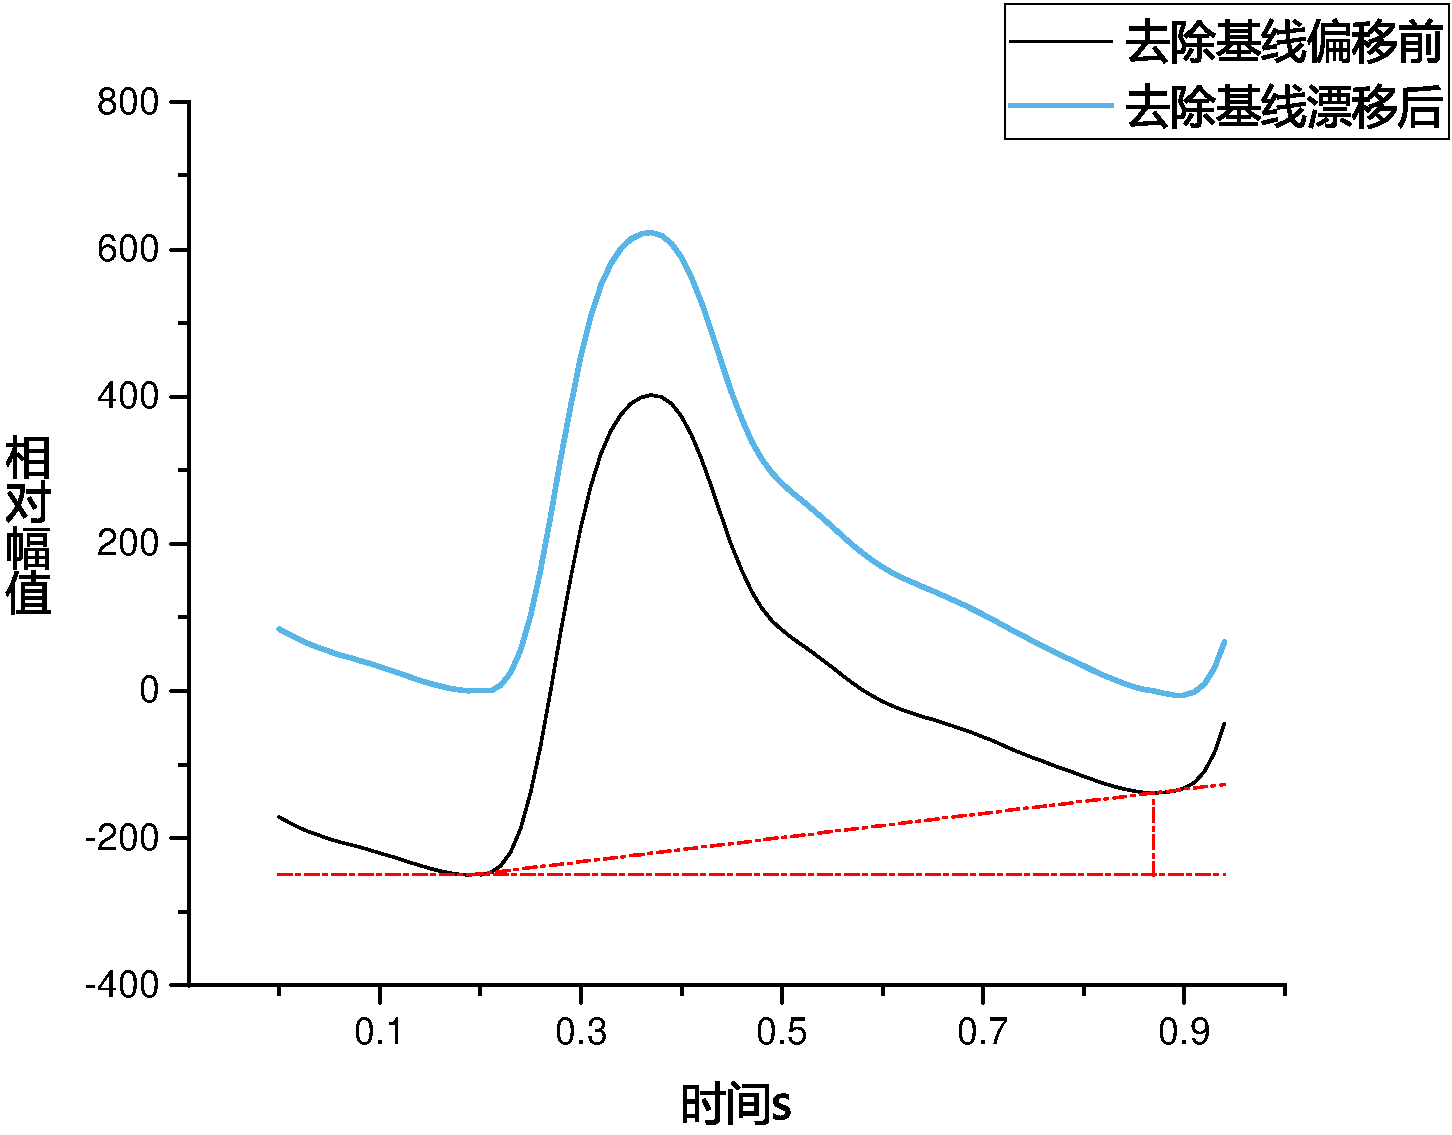
\includegraphics[width=.6\linewidth]{ch4/baselineadjust}
    \caption{\label{fig:drift}基线漂移去除原理示意及处理前后对比}
\end{figure}

如\autoref{fig:drift}所示,易知脉搏波的相对幅值$A$是采样时间$t$的函数,将其表示为$A(t)$。对任一特定波形,其起始点与终止点处对应的幅值可分别表示为$A(t_{start})$与$A(t_{end})$。
由于始末位置脉搏波幅值不等,则明显两者之间存在一条斜率不为0的直线,其具体值为
\begin{equation}
    \label{equ:linek}
    k=\frac{A(t_{start})-A(t_{end})}{t_{start}-t_{end}}
\end{equation}
则该直线上任意点即代表了在该时刻脉搏波波形与水平基线的偏移量,即
\begin{equation}
    \label{equ:liney}
    \Delta(t)=k(t-t_{start})+A(t_{start})
\end{equation}
此时,去除基线漂移后的脉搏波信号可标示为
\begin{equation}
    \label{equ:adjusta}
    A_{adjsut}(t)=A(t)-\Delta(t)
\end{equation}

\subsection{插值计算}
由于本章后部分自行定义设计的多种新型脉搏波特征,在特征计算过程中对脉搏波的采样频率有着较高要求。由于GE B450设备导出的原始脉搏波数据的采集频率仅为100$Hz$,难以满足后续计算。因此,需要在PPG预处理环节额外引入了插值计算操作以人工提高信号采样率。

插值是求值的逆过程,通过某些已知的数据点去推断一个(系列)特定的函数,使得所有已知数据点均在该函数图像上,从而去推断更多未知数据点,解决相应的实际问题,这一过程如\autoref{fig:spline}所示。
\begin{figure}[htbp]
    \centering
    \subfigure[经过点(1,2),(2,1),(4,4)和(5,3)的线性样条]{
    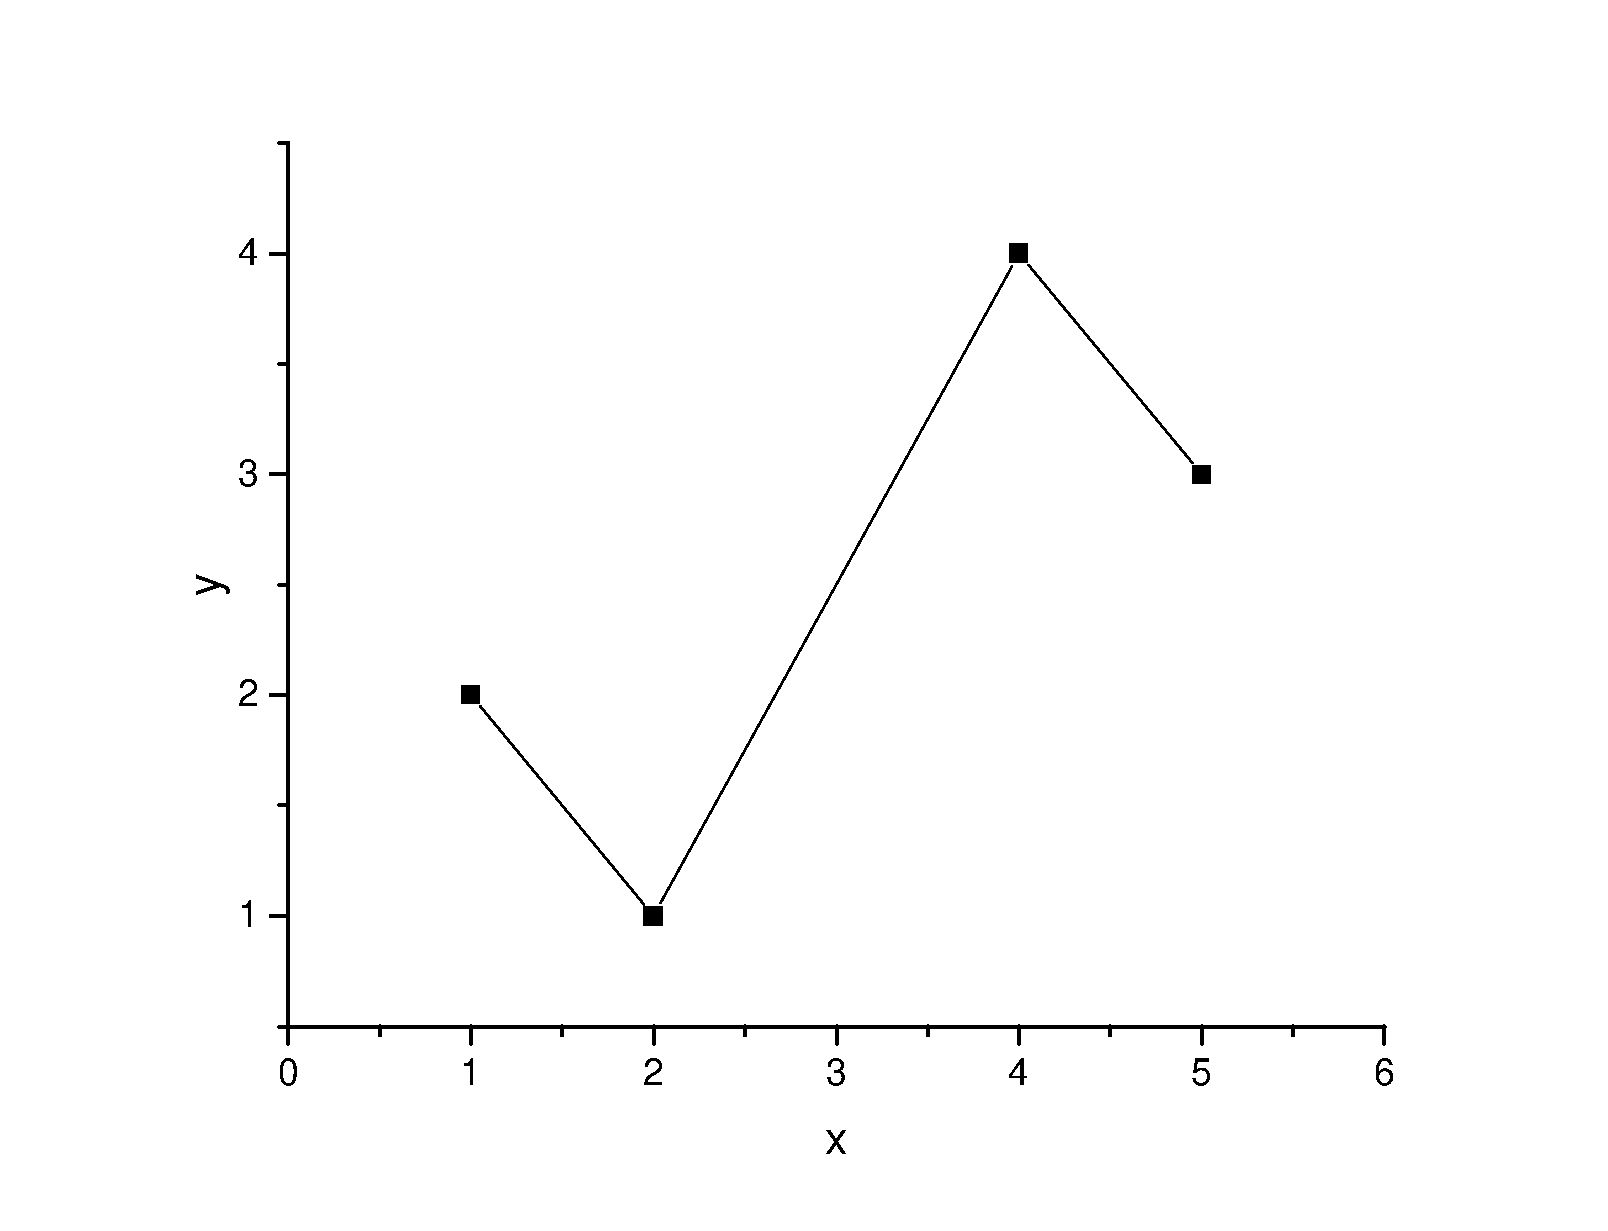
\includegraphics[width=5.5cm]{ch4/spline1}
    }
    \quad
    \subfigure[经过相同点的一种可能的三次样条插值]{
    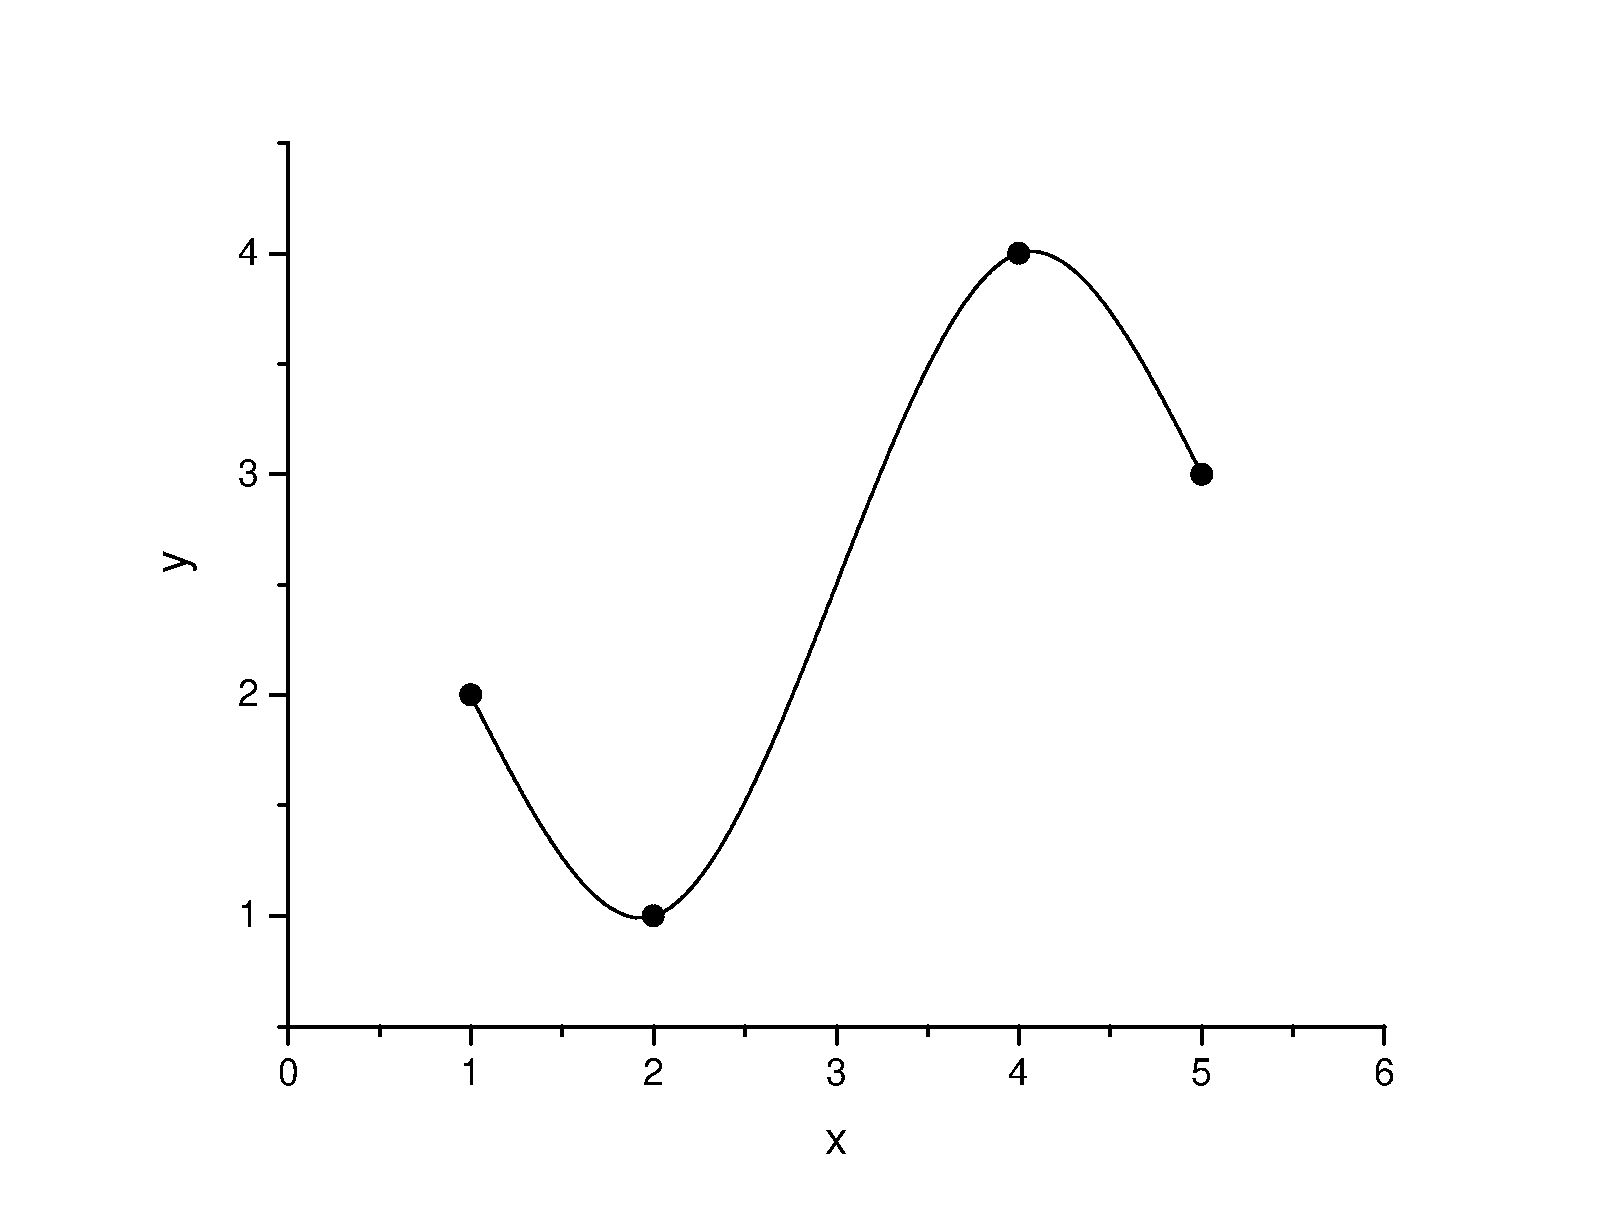
\includegraphics[width=5.5cm]{ch4/spline2}
    }
    \caption{\label{fig:spline}经过4点的线性样条插值与三次样条插值对比}
\end{figure}

多项值插值与样条插值是插值最常用的两种算法\cite{Timothy2018,Carl2008}。多项式插值给出满足所有原始数据点的单一公式,由于此过程中仅涉及浮点数加法与乘法,可以很方便的在PC及嵌入式设备上实现,因而得到广泛应用。
而样条插值则使用多个公式来通过所有数据点,其中每个公式均为低阶多项式。三次样条插值是样条插值在工业领域应用最广泛的算法之一,可以得到光滑的拟合插值曲线。
具体而言,对原始数据点$(x_1,y_1),(x_1,y_1),\cdots,(x_n,y_n)$,三次样条的插值曲线$S(x)$在每两个数据分段区间$[x_i,x_{i+1}]$内均使用三阶多项式
\begin{equation}
    \label{equ:spline}
    S_{i}=y_{i}+b_{i}(x-x_{i})+c_{i}{(x-x_{i})}^2+d_{i}{(x-x_{i})}^3
\end{equation}
并保证每两个多项式在端点(即原始数据点)处不仅数值相等,相应的斜率与曲率均相等,即
\begin{equation}
    \label{equ:cubiccha}
    \left \{
    \begin{aligned}
        S_{i}(x_{i})&=y_i,&\text{i=1,$\cdots$,n-1}\\
        S_{i}(x_{i+1})&=y_{i+1},&\text{i=1,$\cdots$,n-1}\\
        S_{i}^{'}(x_{i-1})&=S_{i}^{'}(x_{i}),&\text{i=2,$\cdots$,n-1} \\
        S_{i}^{''}(x_{i-1})&=S_{i}^{''}(x_{i}),&\text{i=2,$\cdots$,n-1}
    \end{aligned}
    \right.
\end{equation}
使用微积分的定义,将\autoref{equ:spline}代入\autoref{equ:cubiccha}化简整理后,可以得到包含$3n-5$个独立方程的方程组。另一方面,由于每个局部$S_i$中有三个未知参数,一共有$3n-3$个待解参数,则此时由线性代数相关知识可知,该方程组有无穷多组解。
即此时可以构造处无穷多条通过所有数据点$(x_i,y_i)$的样条曲线。因此,需要添加额外的方程对样条曲线进行约束,一般的约束条件都是对样条左右端点处进行限定 ,常见的附加边界条件如\autoref{tab:splinekind}所示\cite{Timothy2018}。
\begin{table}[htbp]
    \centering
    \caption{\label{tab:splinekind}几种常见的三次样条端点条件}
    \begin{tabularx}{\linewidth}{X<{\centering}X<{\centering}}
        \toprule 
        \textbf{样条种类}&\textbf{端点条件}\\
        \midrule 
        自然三次样条&
        $
            S_{1}^{''}(x_{1})=0,
            S_{n-1}^{''}(x_{n})=0
        $
        \\
        曲率调整三次样条&
        $\left \{
        \begin{aligned}
            &S_{1}^{''}(x_{1})=v_1,&v_{1}\neq0\\
            &S_{n-1}^{''}(x_{n})=v_n,&v_{n}\neq0
        \end{aligned}
        \right.
        $
        \\
        钳制三次样条&
        $\left \{
        \begin{aligned}
            &S_{1}^{'}(x_{1})=v_1,&v_{1}\neq0\\
            &S_{n-1}^{'}(x_{n})=v_n,&v_{n}\neq0
        \end{aligned}
        \right.
        $
        \\
        抛物线端点三次样条&
        $
            d_1=0,d_{n-1}=0
        $
        \\
        非纽结三次样条&
        $
            d_1=d_2, d_{n-2}=d_{n-1}
        $
        \\
        \bottomrule
    \end{tabularx}
\end{table}

在补充\autoref{tab:splinekind}中的两个端点条件公式后,即可完成上述方程组求解,从而确定唯一的三次样条插值曲线。本研究中三次样条算法基于自然边界条件对PPG信号进行均匀插值\cite{ttk2021},使信号采样率被提高至2000$Hz$。
\subsection{数据标准化}
在上述各项预处理过程完成后,此时得到的PPG数据在波形幅值上仍然有很大的个体差异,即使对同一被试对象,其波形在幅值上也会有一定的波动。为消除个体差异对特定波形特征计算的影响,需要对脉搏波信号进行归一化处理。

时间标准化与幅值标准化是PPG标准化两类常见的方式\cite{mmt}。时间标准化的基本原理是将PPG信号进行分组并计算每组信号的平均心动周期,随后对每组内的PPG信号进行时间尺度上的缩放,使最终的总平均心动周期保持一致。
由于不同个体的时间尺度上的缩放比例不一致,很容易导致PPG信号波形发生畸变失真,严重影响后续特征计算。故本研究采取了幅值标准化的处理方式对PPG信号进行处理。

由第二章PPG信号光学采集的基本原理可知,PPG信号的波形幅值对不同个体而言并无实际的生理意义,这保证了对PPG信号幅值标准化的合理性。与去除基线漂移过程类似,对待处理的特定PPG波形内所有采样点进行一次线性变换即可完成处理。
为使后续特征计算各项数值不会出现大量的小数,本研究没有采用最常见的归一化处理,而是将单个波形内所有数据点按同一尺度缩放映射到$[0,1000]$区间内。
另一方面,对于同一被试的不同PPG波形而言,其幅值的相对高低变化可能蕴含了一定的生理信息。因此,在标准化过程中,所有波形的标准化系数即缩放比例也同时保存记录下来。

\section{脉搏波的描述}
脉搏波的波形特征变化是评价人体心血管系统生理病理状态的重要依据\cite{PPGYY}。换言之,脉搏波信号携带了能够表征人体心血管系统生理病理状态的全部信息,这些信息蕴藏在了PPG波形的变化之中。
第二章PPG采集原理已经介绍过,PPG信号随机性强,且易受外界干扰,甚至同一个人在不同时间段的脉搏波也不一定相同,如\autoref{fig:pulsecontrast}所示。
因此,当获取到PPG信号的原始数据后,如何对脉搏波进行精确描述成为了一切分析工作的前提。
\begin{figure}[htbp]
    \centering
    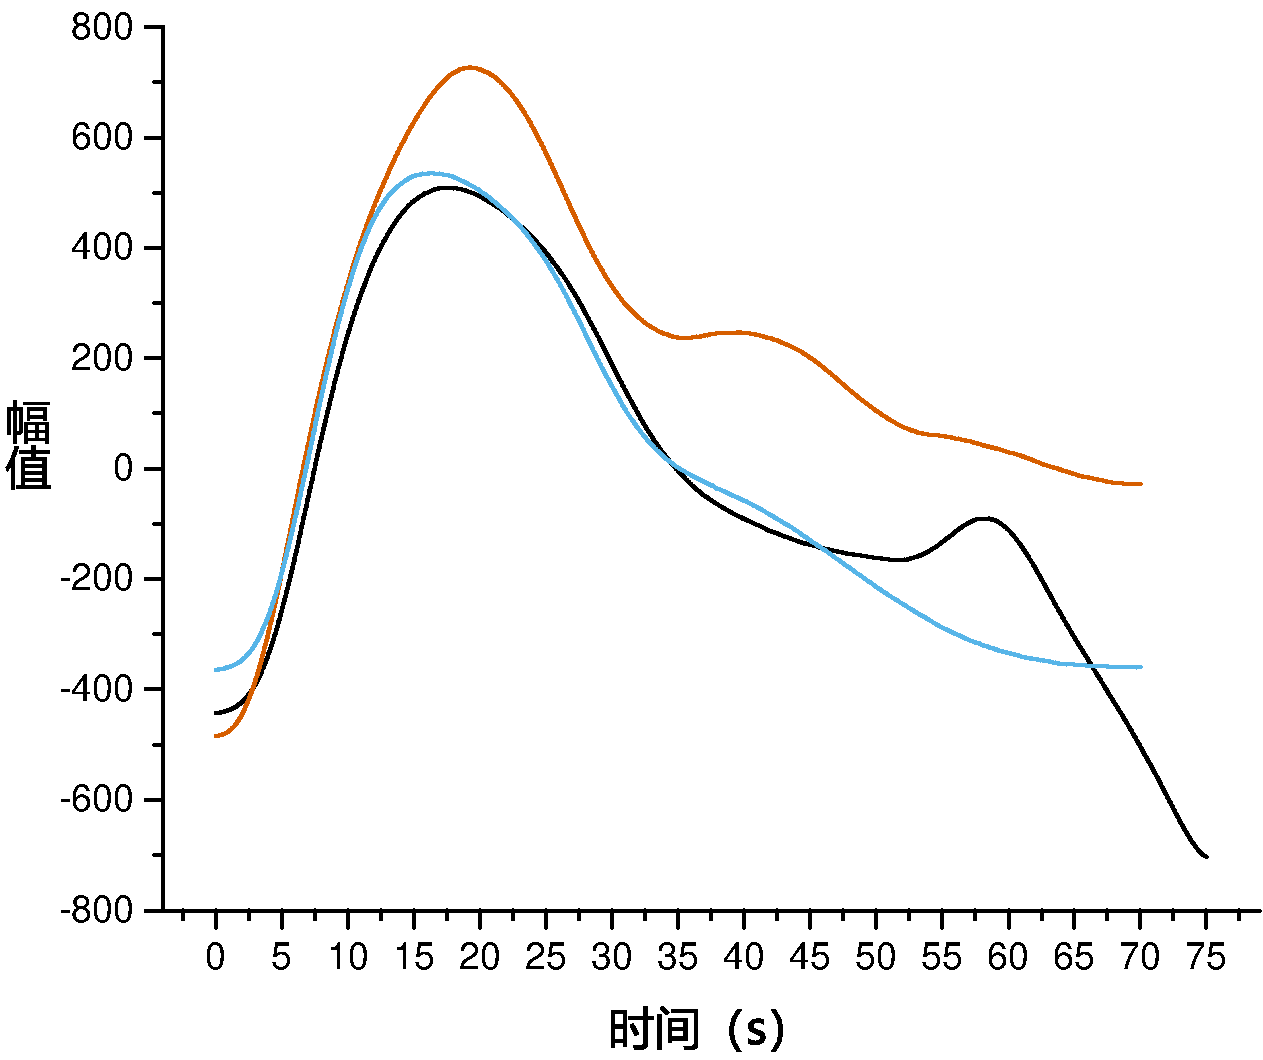
\includegraphics[width=.6\linewidth]{ch4/pulsecontrast}
    \caption[同一名被试PPG信号三段波形对比]{\label{fig:pulsecontrast}同一名被试PPG信号三段波形对比。波形按起点时间对齐,此外无任何其他预处理操作。可以看到三段波形在重搏的显著程度、时长、幅值等方面均有所差异。}
\end{figure}
\subsection{描述的本质}
通信工程中认为,信息是事物运动状态或存在方式的不确定性描述,是通信的内涵;消息是能够被人体感觉器官所感知的物理现象,是信息的外在表现形式;信号则是消息的物理表现形式,是消息的载体\cite{Shannon1948,Liu2019,Zhao2017}。
目前较为常见的完整通讯系统模型如\autoref{fig:communication}所示。其中,信源是产生消息的源头,是通信的起点。信道是信息的传输媒介,是对实际传输过程的抽象,由于信息的传输过程中会难以避免的引入噪声与干扰,
通信工程常将系统各部分所受到的干扰与噪声折合成信道干扰。\autoref{fig:communication}中的编码过程与解码过程则是为保证传输质量与通讯稳定而对消息符号按照预设的规则进行编码与解码工作。
信宿则是信息传输的目的地,也是接收消息的对象,是本次通信的终点\cite{Zhao2017}。
\begin{figure}[htbp]
    \centering
    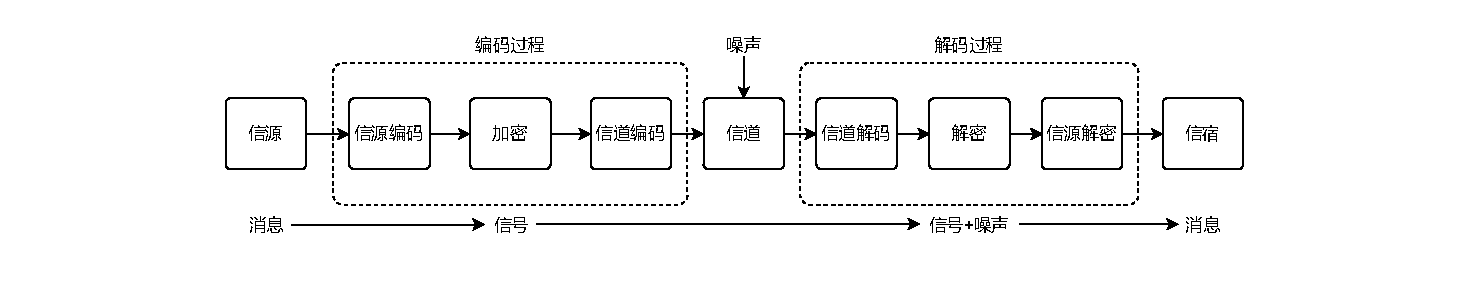
\includegraphics[width=\linewidth]{ch4/communication}
    \caption[通信系统模型框图]{\label{fig:communication}通信系统模型框图\cite{Zhao2017,Liu2019}}
\end{figure}

若从通信原理的角度来看待信号分析的一般过程,那么所有基于人体电生理信号的相关研究均可以抽象地看成特定生理信息从人体或人体某一器官到研究学者、临床医生等之间的信息传输问题,如\autoref{fig:ppgcommunication}所示。
以本研究涉及的脉搏波PPG信号为例,那么搏动不止的心脏显然是这一通讯系统的信源,人体内各脏器系统、组织等可以看成是一个复杂的黑箱编码系统(此部分参见第二章脉搏波产生原理的脉搏波参数模型与非参数模型相关内容)。人体表面丰富的毛细血管则是
该通讯过程中的信道,若因PE等疾病引起了人体毛细血管等系统的生理性变化可以折合成对信道的干扰噪声。而PPG信号本身则是反映信源心脏功能与信道基本特性的消息载体。\textbf{在此基础上,脉搏波的描述过程即可视为在编码规则不明确(黑箱模型)的前提
下对携带上述生理信息的信号进行译码解码的过程。}
\begin{figure}[htbp]
    \centering
    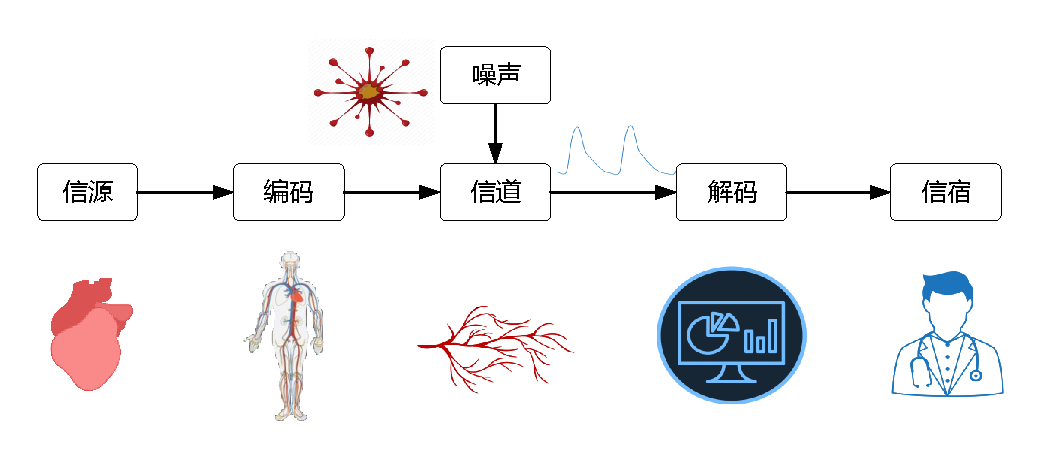
\includegraphics[width=.8\linewidth]{ch4/ppgcommunication}
    \caption{\label{fig:ppgcommunication}以通讯工程的视角看待脉搏波的分析过程}
\end{figure}

另一方面,PPG信号常以一个数字序列表示在一定的采样时间该信号的所有采样值,其序列的长度与信号采样率成正比,一般在100$Hz$以上。而不论是类似“该波形周期较长”、“该波形重播波潮波不明显”等自然语言描述(经过数字标签化处理后),
还是以“下降支时长为0.43s”、“该波形波峰幅值为1351”等绝对量化的数值描述,都是以较少的数值去完成PPG信号的描述与评估过程。\textbf{则显然,上述PPG信号的数字量化过程亦是一个降维处理过程,其本质仍是信息压缩。}

\subsection{常见的脉搏波时域特征}
通常而言,对信号进行分析可以采取时频分析方法。但由于脉搏波频域带宽窄,且本研究采集得到的数据波形较为简单、干扰少、整体质量较高,因此,本研究主要从时域角度对脉搏波进行特征提取与描述工作。
如上小节所述,此前诸多学者提出的多项PPG特征参数就是从不同侧面对原始数据进行数字量化与降维处理的过程。本小节将前人提出的脉搏波时域特征进行了汇总整理,并按特征计算所使用的时长分为基于PPG完整波形与基于(固定)
时间窗(如基于整条数据记录的相关特征)两大类。特别地,对已在子痫前期的相关研究中得到应用的脉搏波(含压力脉搏波)特征参数进行了详细说明。

一、基于波形的时域特征

1. 基于多个波形的特征

脉搏波波形速度(Pulse Wave Velocity,PWV)是指心脏每次搏动射血产生的沿大动脉壁传播的压力波传导速度,常与脉搏波传导时间(Pulse Transit Time,PTT)通用。PWV已被证实与动脉扩张性、僵硬度、管壁厚度和血液黏稠度密切相关。
特别地,PWV已经在子痫前期的诸多研究中得到应用\cite{Tomsin2012,Katsipi2014,VivianaIvan2018,Ira2014}。
但由于PWV检测基本原理依赖于在人体不同部位采用压力传感器检测脉搏波并记录两部位之间的体表距离及PTT,故不适用单点测量的光电容积脉搏波研究。

2. 一维特征

3. 二维特征

SPV

dPP

AIx

PSI

ADR

K


4. 通用无量纲参数与高阶统计量

无量纲参数(non-dimensional parameter)是指不使用计量学中基本单位及导出单位进行衡量的参数,该类参数通常以比值的形式出现,故严格意义来说,前文中部分比值类参数也可划归至无量纲参数中。
无量纲参数作为信号时域分析重要参考指标,在机械控制、石油石化、电信电子、地球物理、故障诊断、信号处理等领域有着广泛的应用\cite{Jardine2006,Guo2014,Tu2013,Mendel1991}。本研究中使用了常见的峰值因子(crest factor)、
脉冲因子(impulse factor)、裕度因子(clearance factor)及波形因子(form factor)等指标对脉搏波信号进行评估,相关参数的基本定义如\autoref{tab:ndp}所示。

高阶统计量(High Order Statitics,HOS)是指非传统的二阶统计量(如时域相关函数、频域功率谱密度等),通常是三阶或三阶以上的统计量\cite{Zhang2002,Tu2013}。高阶统计量是研究分析非线形、非因果、非最小相位系统和非高斯、非平稳、非加性噪声的重要分析工具。
本研究使用了高阶统计量中表示分布的峭度因子(kurtosis factor)与偏度(skewness)对PPG信号进行了评估,两者的基本定义参见\autoref{tab:ndp}。
\begin{table}[htbp]
    \centering
    \caption{\label{tab:ndp}本研究使用的无量纲参数及高阶统计量}
    \begin{tabularx}{\linewidth}{cX<{\centering}c}
        \toprule
        \textbf{参数}&\textbf{物理(统计)意义}&\textbf{定义方程}\\
        \midrule
        峰值因子&信号峰值与信号有效值(均方根值)的比值& $C=\frac{X_{peak}}{X_{RMS}}$      \\
        脉冲因子&信号峰值与信号整流值(绝对值的平均值)的比值&$I=\frac{X_{peak}}{|\bar{X}|}$      \\
        裕度因子&信号峰值与信号方根幅值的比值&$C_e=\frac{X_{peak}}{X_R}$       \\
        波形因子&信号有效值与信号整流值的比值&$S_f=\frac{X_{RMS}}{|\bar{X}|}$      \\
        峭度因子&信号四阶中心矩和信号标准差的四次方的比值&$K_4=\frac{E[(X-\mu)^4]}{\sigma^4}$      \\
        偏度&信号三阶中心矩和信号标准差的三次方的比值&$K_3=\frac{E[(X-\mu)^3]}{\sigma^3}$      \\
        \bottomrule
    \end{tabularx}
\end{table}

从\autoref{tab:ndp}可以发现,峰值因子、脉冲因子、裕度因子具有相似的物理定义,均是信号峰值与原始信号的某一统计量均值进行比较。由数字信号处理的原理可知,均值计算可以看成是一个简单的低通滤波模型,
对突变的脉冲信号有较好的抑制作用。因而,这三个非量纲参数对脉冲冲击导致的峰值变化比较敏感。
而波形因子则是两个统计量均值的比值,对脉冲信号的敏感性不高。另一方面,高阶统计量峭度因子和偏度反应的是原始信号的分布特性,如\autoref{fig:skew}所示。峭度因子常在信号处理中作为高斯信号与非高斯信号的划分标准,高斯信号的峭度因子为3。
偏度则主要反应信号的左右对称性,完全对称的信号其偏度为0。
\begin{figure}[htbp]
    \centering
    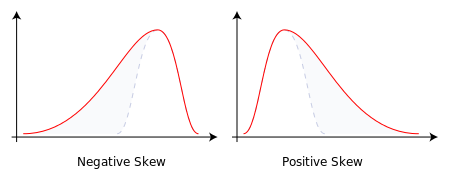
\includegraphics[width=.6\linewidth]{ch4/skew}
    \caption{\label{fig:skew}峭度因子与偏度示意}
\end{figure}

二、基于时间窗的时域特征

\subsection{新型时域特征参数设计}
在总结前人研究基础上,本研究结合脉搏波形态特点,设计了多种新型时域描述参数,以求从新的角度完成对脉搏波波形特征的描述。此外,作为PPG信号最典型特征,重搏波可以在很大程度上反应人体血管外周阻力、血管壁弹性等信息,
但以往的研究对脉搏波的重搏波相关特性描述较少,对重搏波的描述往往局限于“波形特征明显”与“波形特征不明显”等简单文字定性描述,缺乏具体定量描述标准。鉴于此,本研究首创设计了多种量化指标以具体描述PPG信号重搏波形态特征。

一、新型脉搏波时域特征

1. 波形时域特征的设计基础

以纯数学的角度来看,PPG的信号波形可以近似描述为从一条往复于水平基线与波峰之间双向路径。一般而言,PPG信号的上升支通常较下降支更为简单,该双向路径可以进一步简化为从波峰下降至水平基线的一条单向路径,只要完成对该单向路径的描述
即可类比完成上升支的描述,从而完成对整个脉搏波波形的描述。不失一般性,我们可以将下降支的单向路径的起点坐标与终点坐标分别设置为S$(0,1)$与E$(1,0)$,加上坐标原点O$(0,0)$,这一过程如\autoref{fig:road}所示。
\begin{figure}[htbp]
    \centering
    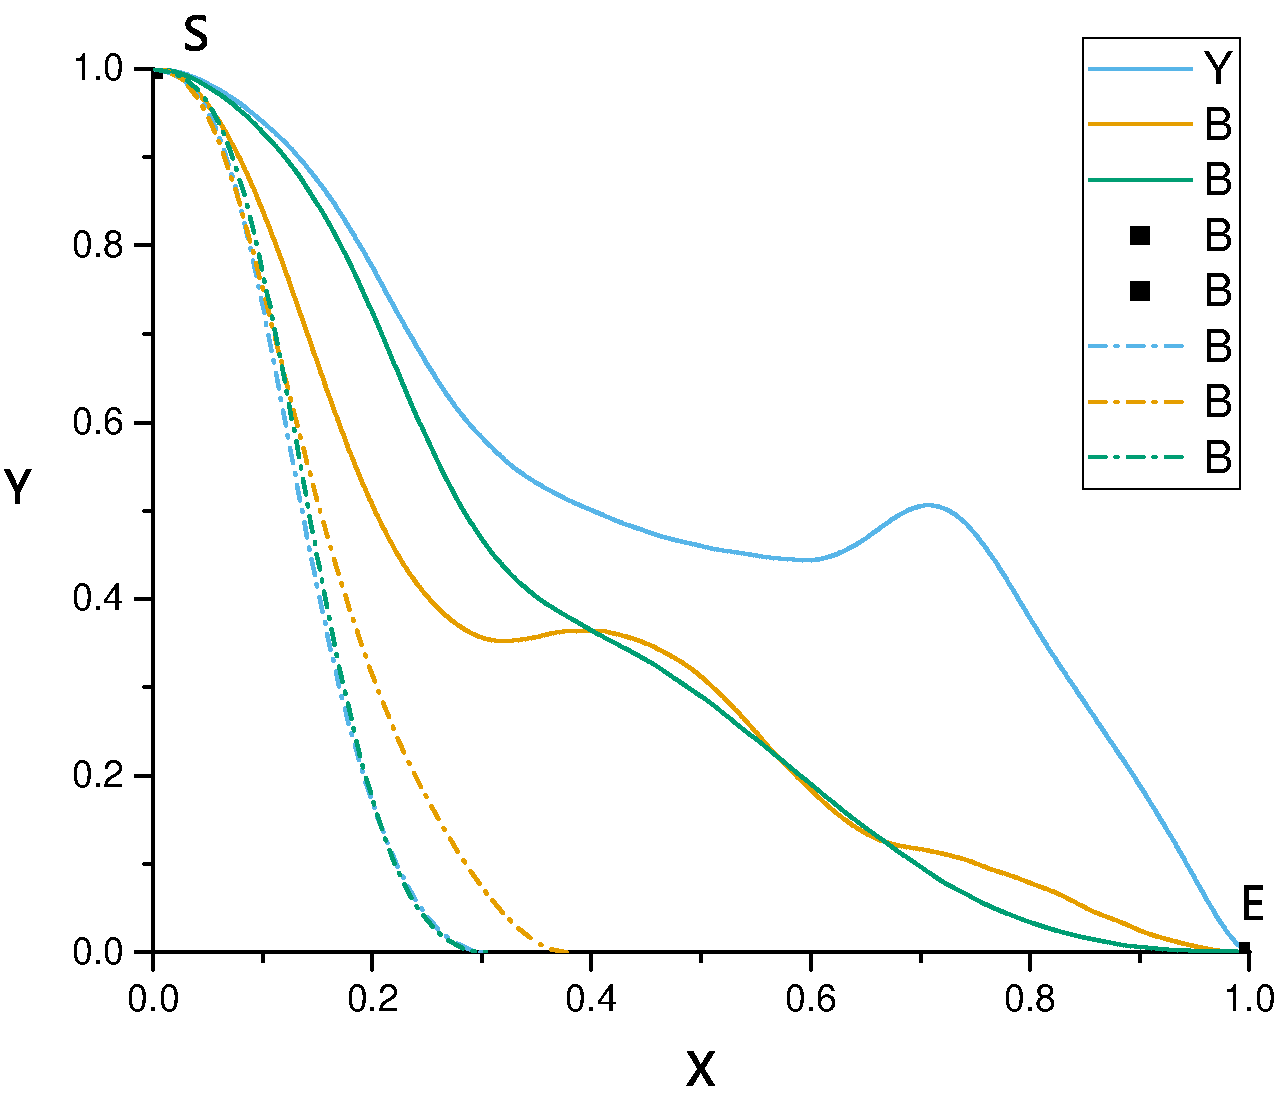
\includegraphics[width=.6\linewidth]{ch4/road2}
    \caption[脉搏波波形的单向路径表示]{\label{fig:road}脉搏波波形的单向路径表示。其中三条路径由\autoref{fig:pulsecontrast}所示的同一被试的三段波形对应线形变换得来。同一颜色的实线部分与虚线部分对应同一个脉搏波的下降支与上升支
    ,其中,下降支按一定比例缩放至目标区间内,上升支水平反向按同一比例反向进行了缩放。}
\end{figure}



2. 角度、幅值、长度等

二、重搏波的量化描述

量化描述重搏波明显程度

\subsection{PPG时域描述特征集构建}
\section{小结}